\documentclass[a4paper]{article}

\usepackage{inputenc}
\usepackage[british,UKenglish]{babel}
\usepackage{amsmath}
%\usepackage{titlesec}
\usepackage{color}
\usepackage{graphicx}
\usepackage{fancyref}
\usepackage{hyperref}
\usepackage{float}
\usepackage{scrextend}
\usepackage{setspace}
\usepackage{xargs}
\usepackage{multicol}
\usepackage{nameref}

\usepackage{sectsty}
\usepackage{multicol}
\usepackage{multirow}
\usepackage[procnames]{listings}
\usepackage{appendix}

\newcommand\tab[1][1cm]{\hspace*{#1}}
\hypersetup{colorlinks=true, linkcolor=black}
\interfootnotelinepenalty=10000

\newcommand{\cleancode}[1]{\begin{addmargin}[3em]{3em}\texttt{\textcolor{cleanOrange}{#1}}\end{addmargin}}
\newcommand{\cleanstyle}[1]{\text{\textcolor{cleanOrange}{\texttt{#1}}}}


\usepackage[colorinlistoftodos,prependcaption,textsize=footnotesize]{todonotes}
\newcommandx{\commred}[2][1=]{\textcolor{Red}
{\todo[linecolor=red,backgroundcolor=red!25,bordercolor=red,#1]{#2}}}
\newcommandx{\commblue}[2][1=]{\textcolor{Blue}
{\todo[linecolor=blue,backgroundcolor=blue!25,bordercolor=blue,#1]{#2}}}
\newcommandx{\commgreen}[2][1=]{\textcolor{OliveGreen}{\todo[linecolor=OliveGreen,backgroundcolor=OliveGreen!25,bordercolor=OliveGreen,#1]{#2}}}
\newcommandx{\commpurp}[2][1=]{\textcolor{Plum}{\todo[linecolor=Plum,backgroundcolor=Plum!25,bordercolor=Plum,#1]{#2}}}

\def\code#1{{\tt #1}}

\def\note#1{\noindent{\bf [Note: #1]}}

\makeatletter
%% The "\@seccntformat" command is an auxiliary command
%% (see pp. 26f. of 'The LaTeX Companion,' 2nd. ed.)
\def\@seccntformat#1{\@ifundefined{#1@cntformat}%
   {\csname the#1\endcsname\quad}  % default
   {\csname #1@cntformat\endcsname}% enable individual control
}
\let\oldappendix\appendix %% save current definition of \appendix
\renewcommand\appendix{%
    \oldappendix
    \newcommand{\section@cntformat}{\appendixname~\thesection\quad}
}
\makeatother


% "define" Scala
\usepackage[T1]{fontenc}  
\usepackage[scaled=0.82]{beramono}  
\usepackage{microtype} 

\sbox0{\small\ttfamily A}
\edef\mybasewidth{\the\wd0 }

\lstdefinelanguage{scala}{
  morekeywords={abstract,case,catch,class,def,%
    do,else,extends,false,final,finally,%
    for,if,implicit,import,match,mixin,%
    new,null,object,override,package,%
    private,protected,requires,return,sealed,%
    super,this,throw,trait,true,try,%
    type,val,var,while,with,yield},
  sensitive=true,
  morecomment=[l]{//},
  morecomment=[n]{/*}{*/},
  morestring=[b]",
  morestring=[b]',
  morestring=[b]"""
}

\usepackage{color}
\definecolor{dkgreen}{rgb}{0,0.6,0}
\definecolor{gray}{rgb}{0.5,0.5,0.5}
\definecolor{mauve}{rgb}{0.58,0,0.82}

% Default settings for code listings
\lstset{frame=tb,
  language=scala,
  aboveskip=3mm,
  belowskip=3mm,
  showstringspaces=false,
  columns=fixed, % basewidth=\mybasewidth,
  basicstyle={\small\ttfamily},
  numbers=none,
  numberstyle=\footnotesize\color{gray},
  % identifierstyle=\color{red},
  keywordstyle=\color{blue},
  commentstyle=\color{dkgreen},
  stringstyle=\color{mauve},
  frame=single,
  breaklines=true,
  breakatwhitespace=true,
  procnamekeys={def, val, var, class, trait, object, extends},
  procnamestyle=\ttfamily\color{red},
  tabsize=2
}

\lstnewenvironment{scala}[1][]
{\lstset{language=scala,#1}}
{}
\lstnewenvironment{cpp}[1][]
{\lstset{language=C++,#1}}
{}
\lstnewenvironment{bash}[1][]
{\lstset{language=bash,#1}}
{}
\lstnewenvironment{verilog}[1][]
{\lstset{language=verilog,#1}}
{}



%代码段设置
\lstset{numbers=left,
basicstyle=\tiny,
numberstyle=\tiny,
keywordstyle=\color{blue!70},
commentstyle=\color{red!50!green!50!blue!50},
frame=single, rulesepcolor=\color{red!20!green!20!blue!20},
escapeinside=``
}

\graphicspath{ {images/} }
\usepackage{ctex}
\usepackage{graphicx}
\usepackage{color,framed}%文本框
\usepackage{listings}
\usepackage{caption}
\usepackage{amssymb}
\usepackage{enumerate}
\usepackage{xcolor}
\usepackage{bm} 
\usepackage{lastpage}%获得总页数
\usepackage{fancyhdr}
\usepackage{tabularx}  
\usepackage{geometry}
\usepackage{minted}
\usepackage{graphics}
\usepackage{subfigure}
\usepackage{float}
\usepackage{pdfpages}
\usepackage{pgfplots}
\pgfplotsset{width=10cm,compat=1.9}
\usepackage{multirow}
\usepackage{footnote}
\usepackage{booktabs}

%-----------------------伪代码------------------
\usepackage{algorithm}  
\usepackage{algorithmicx}  
\usepackage{algpseudocode}  
\floatname{algorithm}{Algorithm}  
\renewcommand{\algorithmicrequire}{\textbf{Input:}}  
\renewcommand{\algorithmicensure}{\textbf{Output:}} 
\usepackage{lipsum}  
\makeatletter
\newenvironment{breakablealgorithm}
  {% \begin{breakablealgorithm}
  \begin{center}
     \refstepcounter{algorithm}% New algorithm
     \hrule height.8pt depth0pt \kern2pt% \@fs@pre for \@fs@ruled
     \renewcommand{\caption}[2][\relax]{% Make a new \caption
      {\raggedright\textbf{\ALG@name~\thealgorithm} ##2\par}%
      \ifx\relax##1\relax % #1 is \relax
         \addcontentsline{loa}{algorithm}{\protect\numberline{\thealgorithm}##2}%
      \else % #1 is not \relax
         \addcontentsline{loa}{algorithm}{\protect\numberline{\thealgorithm}##1}%
      \fi
      \kern2pt\hrule\kern2pt
     }
  }{% \end{breakablealgorithm}
     \kern2pt\hrule\relax% \@fs@post for \@fs@ruled
  \end{center}
  }
\makeatother
%------------------------代码-------------------
\usepackage{xcolor} 
\usepackage{listings} 
\lstset{ 
breaklines,%自动换行
basicstyle=\small,
escapeinside=``,
keywordstyle=\color{ blue!70} \bfseries,
commentstyle=\color{red!50!green!50!blue!50},% 
stringstyle=\ttfamily,% 
extendedchars=false,% 
linewidth=\textwidth,% 
numbers=left,% 
numberstyle=\tiny \color{blue!50},% 
frame=trbl% 
rulesepcolor= \color{ red!20!green!20!blue!20} 
}

%-------------------------页面边距--------------
\geometry{a4paper,left=2.3cm,right=2.3cm,top=2.7cm,bottom=2.7cm}
%-------------------------页眉页脚--------------
\usepackage{fancyhdr}
\pagestyle{fancy}
\lhead{\kaishu \leftmark}
% \chead{}
\rhead{\kaishu 并行程序设计实验报告}%加粗\bfseries 
\lfoot{}
\cfoot{\thepage}
\rfoot{}
\renewcommand{\headrulewidth}{0.1pt}  
\renewcommand{\footrulewidth}{0pt}%去掉横线
\newcommand{\HRule}{\rule{\linewidth}{0.5mm}}%标题横线
\newcommand{\HRulegrossa}{\rule{\linewidth}{1.2mm}}
\setlength{\textfloatsep}{10mm}%设置图片的前后间距
%--------------------文档内容--------------------

\begin{document}
\renewcommand{\contentsname}{目\ 录}
\renewcommand{\appendixname}{附录}
\renewcommand{\appendixpagename}{附录}
\renewcommand{\refname}{参考文献} 
\renewcommand{\figurename}{图}
\renewcommand{\tablename}{表}
\renewcommand{\today}{\number\year 年 \number\month 月 \number\day 日}

%-------------------------封面----------------
\begin{titlepage}
    \begin{center}
    
\includegraphics[width=0.8\textwidth]{NKU.png}\\[1cm]
    \vspace{20mm}
		\textbf{\huge\textbf{\kaishu{计算机学院}}}\\[0.5cm]
		\textbf{\huge{\kaishu{数据库第一次作业报告}}}\\[2.3cm]
		\textbf{\Huge\textbf{\kaishu{cmu15445 protect0+protect1}}}

		\vspace{\fill}
    
    % \textbf{\Large \textbf{并行程序设计期末实验报告}}\\[0.8cm]
    % \HRule \\[0.9cm]
    % \HRule \\[2.0cm]
    \centering
    \textsc{\LARGE \kaishu{姓名\ :\ 孔德嵘}}\\[0.5cm]
    \textsc{\LARGE \kaishu{学号\ :\ 2213626}}\\[0.5cm]
    \textsc{\LARGE \kaishu{专业\ :\ 计算机科学与技术}}\\[0.5cm]
    
    \vfill
    {\Large \today}
    \end{center}
\end{titlepage}

\renewcommand {\thefigure}{\thesection{}.\arabic{figure}}%图片按章标号
\renewcommand{\figurename}{图}
\renewcommand{\contentsname}{目录}  
\cfoot{\thepage\ of \pageref{LastPage}}%当前页 of 总页数


% 生成目录
\clearpage
\tableofcontents
\newpage

\section{前言}

CMU 15-445是卡内基梅隆大学(Carnegie Mellon University)的数据库系统课程。

所有的project在BusTub数据库管理系统上编写,所有代码使用C++编写,并且使用了
C++17特性,包括智能指针、锁和线程、强制类型转换等新特性。另外需要注意的是,
每次提交任务时需要检查代码规范性和可读性,不然Vscode会进行报错,甚至存在编译无法通过
的情况。

每个任务完成时会提交至\href{https://github.com/aakennes/Database}{仓库},提交方式:

\begin{minted}[mathescape,
   linenos,
   numbersep=5pt,
   gobble=2,
   frame=lines,
   framesep=2mm,
   highlightcolor=green!40]{bash}
   git add .
   git commit -m "xxx"
   git push -u origin main
\end{minted}

笔者所使用的环境如下:

\begin{table}[h!]
   \begin{tabular}{|l|l|l|}
   \hline
   编译器            & 代码编辑器      & 操作系统               \\  \hline
   clang++ 14.0.0 & vscode ssh & linux ubuntu 22.04 \\  \hline
   \end{tabular}
\end{table}

编译及单步测试指令如下:

\begin{minted}[mathescape,
   linenos,
   numbersep=5pt,
   gobble=2,
   frame=lines,
   framesep=2mm,
   highlightcolor=green!40]{bash}
   cmake -DCMAKE_BUILD_TYPE=Debug ..
   # 本地运行时使用Debug模式,上传时使用Release模式,检查内存时添加-DBUSTUB_SANITIZER=
   make orset_test -j$(nproc)
   ./test/orset_test
   # orset_test换成对应任务的测试名
\end{minted}

(Vscode同样具有测试选项,相较本地终端运行较为方便,可以运行单步测试的某个
测试点)

经过测试,在三个模式下均可通过所有测试点(Project1 task4通过网上样例进行了加强),
且没有内存泄漏问题。但是存在一个小问题,在运行test可执行文件时会有20\%的概率报段错误
(SegmentError),且未查明原因。

在Debug时发现编译器对编译影响较大,笔者之前使用Clang++15.0.7,在编译
Project1时遇到很严重的编译问题,例如:unqualified call to 'std::move'
[-Werror,-Wunqualified-std-cast-call],若有相关编译问题需检查编译版本,
并通过如下方式检查并切换编译器:

\begin{minted}[mathescape,
   linenos,
   numbersep=5pt,
   gobble=2,
   frame=lines,
   framesep=2mm,
   highlightcolor=green!40]{bash}
   sudo update-alternatives --config clang
   sudo update-alternatives --config clang++
\end{minted}


\section{Protect0 - C++ PRIMER}

Project0相对Project1简单很多,实验目的主要是熟悉编译器、工程调试、auto类型和C++17环境(新特性中的
强制类型转换和智能指针),同时还需熟悉\href{https://google.github.io/styleguide/cppguide.html}{Google C++ Style Guide}的码风,
并与之保持一致,码风差距过大导致make format无法拯救时,会出现编译问题。

\subsection{Task1:OR-Set}

\subsubsection{任务介绍}

本task要求实现一个无冲突数据类型(CRDT:Conflict-free replicated data type),
即OR-Set。

无冲突数据类型是为分布式系统设计的数据结构,是一种可以在网络中的多台计算机上复制的数据结构,
副本可以独立和并行地更新,不需要在副本之间进行协调,并保证不会有冲突发生,保证了
数据库插入信息时的一致性(最终一致性)。

OR-Set是一种基于版本向量的无冲突数据类型,用于实现集合的合并,主要负责处理集合中元素的添加和移除。
每个集合中的元素是二元组,包括元素本身内容(下简称为内容)和Uid两部分,集合中每个元素均不相同,由Uid区分开(即使插入了同样的
内容,Uid不相同也会导致元素不相同)。

OR-Set由两个集合组成,分别是元素集合element\_set\_和墓地集合tomb\_set\_,代表
当前元素集合和已删除元素集合。当一个元素从element\_set\_中移除时,需要进入到tomb\_set\_。
已删除的元素将不会再次添加到element\_set\_中,具体逻辑见代码分析。

主要需要实现添加、删除、合并三个操作,包含五个函数,Add(element,uid)、
Remove(element)、Merge(element)以及判断元素是否在集合中的Contain(elem)
和输出element\_set\_全部元素的Elements()。

\subsubsection{任务分析}

在官方文档中提供了Add、Remove、Merge三个函数的逻辑实现,实现起来相对
容易。需要注意的是,Add和Remove函数操作的对象均为内容,而非元素二元组,
但是元素集合element\_set\_和墓地集合tomb\_set\_里存放的是元素二元组。

先介绍一下以下伪代码中集合运算的一些符号。

\begin{itemize}
   \item[$\cdot$] $E$ 表示元素集合element\_set\_
   \item[$\cdot$] $T$ 表示墓地集合tomb\_set\_
   \item[$\cdot$] $element$ 表示要插入的内容,非二元组元素
   \item[$\cdot$] $n$ 表示二元组的Uid
   \item[$\cdot$] $unique()$ 表示内容生成的Uid
   \item[$\cdot$] $\{(e,n)\}$ 表示由元素(e,n)组成的集合
   \item[$\cdot$] $\backslash$ 表示集合减法,即
      $$ A\backslash B = A \cap ~B $$
\end{itemize}

三个函数的实现逻辑:

\begin{breakablealgorithm} 
   % \caption{初始化obj文件信息——对应MeshSimplify类中readfile函数,Face类calMatrix函数} 
   \begin{algorithmic}[1] %每行显示行号  
       \Require 要插入的内容
      %  \Ensure 是否读取成功
       \Function {add}{$element$}  
               \State let $n = unique() $
               \State $E:=E\cup{\{(e,n)\}}\backslash T$
       \EndFunction
   \end{algorithmic}  
\end{breakablealgorithm}

\begin{breakablealgorithm} 
   % \caption{初始化obj文件信息——对应MeshSimplify类中readfile函数,Face类calMatrix函数} 
   \begin{algorithmic}[1] %每行显示行号  
         \Require 要删除的内容
      %  \Ensure 是否读取成功
         \Function {remove}{$element$}  
               \State let $R = \{(e,n)\|\exists n ,s.t.(e,n)\in E \} $
               \State $E:=E \backslash R$
               \State $T:=T \cup R$
         \EndFunction
         \State 只要E中存在与给定内容相同的二元组,就无视Uid进行全部删除
         \State 需要注意的是,所有具有该内容的二元组都需要删除
         % \Return True
   \end{algorithmic}  
\end{breakablealgorithm}

\begin{breakablealgorithm} 
   % \caption{初始化obj文件信息——对应MeshSimplify类中readfile函数,Face类calMatrix函数} 
   \begin{algorithmic}[1] %每行显示行号  
         \Require 要合并的集合
      %  \Ensure 是否读取成功
         \Function {merge}{$B$}  
               \State $E=(E\backslash B.T)\cup(B.E\backslash T)$
               \State $T=T \cup B.T$
         \EndFunction
         \State 合并B集合前需要检查B的墓地集合,保证合并后的元素集合与墓地集合没有交集
         % \Return True
   \end{algorithmic}  
\end{breakablealgorithm}

\subsubsection{具体实现}

在orset.h中需要我们自己实现两个集合,这里采用vector模拟两个集合,
vector里存有元素二元组,其他五个函数需要再orset.cpp中实现。

\begin{minted}[mathescape,
   linenos,
   numbersep=5pt,
   gobble=2,
   frame=lines,
   framesep=2mm,
   highlightcolor=green!40]{cpp}
   std::vector<std::pair<T, uid_t> > elements_set_;  // set E
   std::vector<std::pair<T, uid_t> > tomb_set_;      // set T
\end{minted}

在构造集合E和T时,采用二分插入和查找的方式,通过algorithm库中的lower\_bound函数
实现二分插入的功能,使得两个集合元素有序,即通过vector+lower\_bound函数对STL中的set
进行了模拟,但是由于vector中存元素的方式是连续的,所以即便使用vector二分查找和插入
元素的过程是O($log_n$)的,在删除时只能调用erase函数实现O(n)的效率。

\begin{minted}[mathescape,
   linenos,
   numbersep=5pt,
   gobble=2,
   frame=lines,
   framesep=2mm,
   highlightcolor=green!40]{cpp}
   auto it = std::lower_bound(elements_set_.begin(), elements_set_.end(), std::pair(elem, static_cast<uid_t>(0)));
   //集合的二分查找
   elements_set_.insert(it, std::pair(elem, uid));
   elements_set_.erase(it);
   //二分插入和普通删除
\end{minted}

bool Contains(elem):
      在elements\_set\_中二分查找内容elem是否存在      

void Add(elem, uid):
      先在tomb\_set\_中查找该元素二元组,如果没查找失败即tomb\_set\_中不存在
      该元素,就在elements\_set\_中二分插入该元素二元组

void Remove(elem):
      在elements\_set\_ 循环查找内容为elem的元素二元组,如果能找到集合中存在
      二元组,则插入到tomb\_set\_中,并删除elements\_set\_中的对应元素。重复
      上述操作至elements\_set\_中找不到内容为elem的元素二元组为止。

void Merge(set):
      这个函数需要注意执行的顺序,我的实现是先将this->elements\_set\_中存在的
      B.tomb\_set\_的元素二元组进行删除,再合并两个elements\_set\_和
      tomb\_set\_。合并elements\_set\_时检查要合并的B.elements\_set\_中的元素二元组
      是否在this->tomb\_set\_。注意,这里由于B集合传递的是地址,尽量不用去
      删除B中的元素二元组。

vector Elements():
      新建一个vector并使用Reserve函数(参数为elements\_set\_.size())进行初始化,
      不进行初始化会产生代码规范问题而报错,将elements\_set\_中的所有元素存入
      vector并进行返回。

\subsubsection{Debug}

\begin{enumerate}
   \item Remove()函数中循环删除元素,原先实现为在循环删除迭代器内的元素后,
   对迭代器进行自增操作,这是一个常见的迭代器删除问题,由于迭代器在
   内存中存储是类似链表式的连续的,当前迭代器内的元素被删除后,下一迭代器的元素会
   补充到当前迭代器上,此时再进行自增会跳过一个迭代器进行访问,最终导致
   访问end()迭代器,报错指针悬空的问题。
   \item 代码规范性问题,强转数据类型需要使用static\_cast函数,除此之外还要
   注意变量名和函数名规范。
 \end{enumerate}

\subsection{Task2:SQL String Functions}

\subsubsection{任务介绍}

实现upper和lower函数,需要分别实现string\_expression.h的Compute函数
和plan\_func\_call.cpp内的GetFuncCallFromFactory函数。

Compute函数要求将给定字符串按照StringExpression类内的成员:StringExpressionType
进行大小写转换。GetFuncCallFromFactory要求我们在排除非法情况后调用
Compute函数进行大小写转换,并通过指针指针进行返回。

\subsubsection{任务分析}

两个函数都较为简单。

\subsubsection{具体实现}

void Compute(\&val):直接逐字符进行大小写转换即可,注意由于
传入的参数是const类型指针,所以无法直接对val进行大小写转换,需要另外
增设string类型变量。


AbstractExpressionRef GetFuncCallFromFactory(\&func\_name, args):
    参数func\_name表示要转换为大写还是小写,args要求大小为1,AbstractExpressionRef是
    Compute()所属类StringExpression的父类。需要注意,通过第二个测试样例可以发现传入的
    参数不合法包括传入参数不为string类型的情况,需要进行判断。



\subsubsection{Debug}

判断参数是否为string类型需要使用AbstractExpressionRef提供的函数GetReturnType()
以及bustub提供的变量类型TypeId::VARCHAR,而非使用typeid()相等进行判断。

\begin{minted}[mathescape,
   linenos,
   numbersep=5pt,
   gobble=2,
   frame=lines,
   framesep=2mm,
   highlightcolor=green!40]{cpp}
   args[0]->GetReturnType().GetType() != TypeId::VARCHAR
\end{minted}

\section{Protect1 - BUFFER POOL}

在这个project中,我们将完整的构造一个面向磁盘的存储管理器,具体而言就是
实现一个缓存池(buffer pool)。

缓存池负责在主存和磁盘之间来回移动物理页,通过物理页和虚拟页的管理,
提高数据访问速度并减少磁盘I/O操作。缓存池主要包括数据页(page),
数据页框架(frame),页面置换系统(Replacer),磁盘调度系统(Diskmanager/Diskscheduler)
,缓存池管理系统(BufferPoolManager),以及线程保护和锁几个部分。
page和frame已经由bustub实现,剩下的四件事分别对应四个task。

这里还需要理清BufferPool的结构,整个BufferPool是处在内存中的。

\begin{figure}[h!]
   \centering
   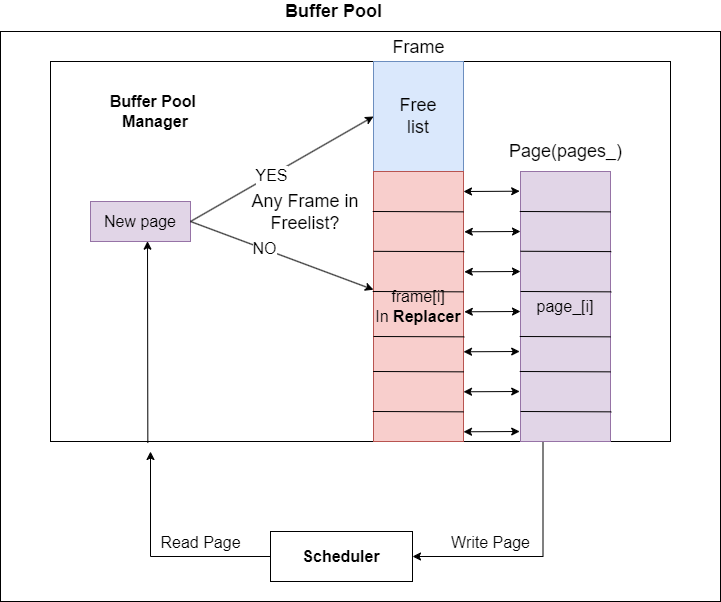
\includegraphics[scale=0.5]{1.png}
   \caption{Buffer Pool的结构}
   \label{fig:1}
\end{figure}

简要逻辑:当数据库系统需要从磁盘(Disk)中通过磁盘调度系统(Diskscheduler)向内存中写入一个新的数据页(page)或者
从数据库系统的磁盘中读取一个内存中的数据页时,要先经过磁盘调度系统传入缓存池(BufferPool),以保证
线程安全。接下来的操作均在缓存池管理系统(BufferPoolManager)中进行,
在缓存池(BufferPool)中新建一个数据页(page)时,会先行检查
数据页框架(frame)中有没有空余的,即Freelist中有无空余框架,
否则就检查页面置换系统(Replacer)有无需要被置换出的框架,BufferPoolManager
中的其他操作也类似。框架和数据页是一一对应的关系,在BufferPoolManager中,pages\_代表数据页,其下标
就是框架的序号。

其中线程保护和锁的一部分是task4的内容,包含在BufferPoolManager中,
具体各个步骤的实现以及内部逻辑将会在下面四个task里面介绍。

\subsection{Task1:LRU-K Replacement Policy}

\subsubsection{任务介绍}

由于内存和硬盘之间读写速度的巨大差异,并且存在程序局部性原理。
页面置换系统又称缓存驱除算法,缓存驱逐算法用于管理在有限的缓存空间中
的数据(数据库系统中的数据页)保留和移除,通过保护将从硬盘中读取出的东西在内存中。
相对于磁盘,在内存里进行操作可以优化缓存的利用率,减少对慢速存储磁盘的访问,
提高CPU的利用率和处理速度。但是由于内存大小局限性,能够申请到的
内存大小远不如磁盘里数据总体的大小,因此需要对数据进行驱逐和置换,
怎样对数据进行驱逐和置换,就涉及到了不同页面置换系统的问题了。

在task1中我们要实现页面置换系统,使用的驱逐算法是LRU-k。需要我们实现
LRU-k的驱逐操作Evict(),历史记录更新RecordAccess(),框架内容数据页移除
Remove(),SetEvictable()设置驱逐标记,总共四个操作。

\subsubsection{任务分析}

LRU-k是LRU的升级版,LRU全称Least Recently Used,译为最近最少使用,
LRU基于这样一个假设:如果数据页最近被访问过,
那么它将来也很可能被访问。因此,当需要在内存中替换一个数据页以空余出
一个新框架时,LRU算法会选择最长时间未被访问的页面并将其淘汰。

LRU-k则不仅考虑了数据页最后一次被访问的时间,还与数据页过去k次访问有关。
LRU-k将处在页面置换系统中与框架对应的数据页分成了两个序列,访问次数少于
k的框架,和访问次数大于等于k的框架。注意在LRU-k中为了方便操作,并
避免对数据页内的数据造成干扰,我们表面上只对框架进行操作,并将框架的各个
信息结合成一个类:LRUKNode,其中包括框架访问历史(链表history\_),框架序号(fid\_)
是否要被驱逐(is\_evictable\_)和k的大小,框架访问历史保存每次访问的时间(时间戳)。

k-distance是决定驱逐顺序的关键,对于框架访问次数少于k的框架,k-distance是
+inf,框架首次访问越早的越先被驱逐。对于框架访问次数大于等于k的框架,k-distance是
倒数第k次访问的时间,k-distance越小的越先被驱逐。对于两个序列,优先对
访问次数少于k的序列进行驱逐操作。

为了方便操作,我们对框架访问次数少于k的k-distance的定义进行修改,修改为
框架第一次访问时间,这样如果小于k和大于等于k的两个序列是分别根据k-distance
排序的,那么就会优先驱逐序列中的首元素。

驱逐顺序:
\begin{enumerate}
   \item 若小于k序列不为空,驱逐小于k序列中的首元素
   \item 若小于k序列为空,驱逐大于等于k序列中的首元素
 \end{enumerate}


 \begin{figure}[htbp]
   \centering
   \begin{minipage}[t]{0.48\textwidth}
      \centering
      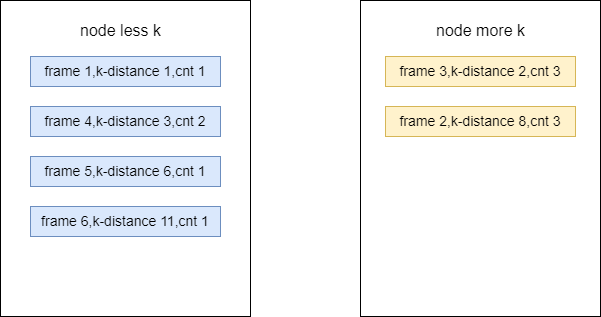
\includegraphics[width=7cm]{2.png}
      \caption{刷新frame4前}
   \end{minipage}
   \begin{minipage}[t]{0.48\textwidth}
      \centering
      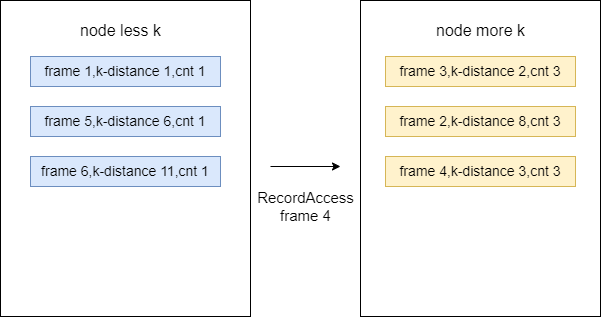
\includegraphics[width=7cm]{3.png}
      \caption{刷新frame4后}
   \end{minipage}
\end{figure}

框架访问顺序:134435322624

以图3.2,3.3为例,其中cnt表示历史访问次数,当使用RecordAccesss刷新frame4时,
frame4的历史访问次数变为了3,需要进入到另一个序列,k-distance为倒数第k次访问时间。
当进行驱逐操作时,驱逐顺序为156324。

\subsubsection{具体实现}

因为在此前我们已经对访问次数小于k的框架的k-distance的定义进行了修改,
使得每次驱逐只需要判断第一个序列是否为空,并删除序列的首元素,前提是能保证
序列中按照k-distance有序。所以对两个序列的实现使用了STL中的集合set,
并进行实时更新。由于驱逐时只能驱逐有驱逐标记的框架,所以比较函数中
要以is\_evictable\_为第一关键字,k-distance为第二关键字进行排序。

两个序列的定义及比较函数的书写:
\begin{minted}[mathescape,
   linenos,
   numbersep=5pt,
   gobble=2,
   frame=lines,
   framesep=2mm,
   highlightcolor=green!40]{cpp}
   struct CompareNode {
    auto operator()(const std::shared_ptr<LRUKNode> &A, const std::shared_ptr<LRUKNode> &B)-> bool {
      return A->is_evictable_ == B->is_evictable_ ? A->history_.front() < B->history_.front()
      : static_cast<int>(A->is_evictable_) > static_cast<int>(B->is_evictable_);
    }
  };
      std::set<std::shared_ptr<LRUKNode>, CompareNode> node_less_k_;
      std::set<std::shared_ptr<LRUKNode>, CompareNode> node_more_k_;
\end{minted}

对于访问历史记录的维护,当访问历史记录(history\_.size())小于k时,每访问一次就pushback一次,
当访问历史记录大于k时,每访问一次除了要pushback外,还需要将队首元素弹出,
保证存储的访问历史记录(history\_.size())一直等于k,这样history\_.front()
就等于k-distance。

线程安全上,由于不需要自己解锁,采用在每个函数(size()除外)前加一把大锁
的方式上锁,使用的锁为C++17中可以自动解锁的scoped\_lock。

时间复杂度上,全部采用了set进行查找插入删除,四个函数的时间复杂度均为
O($log_n$)。

下面是各个函数的实现逻辑:

bool Evict(frame\_id\_t *frame\_id):先判断node\_less\_k\_中是否有
is\_evictable\_=1,即可以驱逐的元素,有就进行驱逐,没有则查看node\_more\_k\_中
是否有可以驱逐的元素。如果两个集合都不存在可以驱逐的元素,返回false,代表
驱逐失败,否则返回true,代表驱逐成功,若驱逐成功,则把驱逐的元素的frame\_id赋值
给函数参数。

node\_store\_存储着frameid与frame信息(LRUKNode)的对应关系,
驱逐一个元素要包括在对应序列里删除该元素,清空历史记录,
删除node\_store\_中的对应关系,最后更新可驱逐元素个数(curr\_size\_)
四个步骤,例如驱逐node\_mode\_k中的一个元素如下:

\begin{minted}[mathescape,
   linenos,
   numbersep=5pt,
   gobble=2,
   frame=lines,
   framesep=2mm,
   highlightcolor=green!40]{cpp}
      node_more_k_.erase(node_more_k_.begin());
      node_store_[*frame_id]->history_.clear();
      node_store_.erase(*frame_id);
      curr_size_--;
\end{minted}

void RecordAccess(frame\_id):更新一个框架的历史记录。按以下步骤进行:
\begin{enumerate}
   \item 在node\_store\_中查找框架是否有对应关系,如果没有就新建一个
   对应关系(LRUKNode),并插入到node\_less\_k(若k=1则插入到node\_more\_k)中。
   \item 如果有对应关系,则判断框架的刷新次数:
   \begin{enumerate}
      \item 刷新次数小于k,更新框架后插入到node\_less\_k中
      \item 刷新次数等于k,先将node\_less\_k内的旧框架进行删除,
      更新框架后再插入到node\_more\_k
      \item 刷新次数等于k,更新框架后插入到node\_more\_k中
   \end{enumerate}
\end{enumerate}

bool SetEvictable(frame\_id,set\_evictable):更新一个框架的is\_evictable\_状态,
注意更新curr\_size\_的大小。同时由于set里面存的是const指针,必须将
node\_less\_k\_和node\_more\_k\_中的值取出来再进行更新,详间Debug。

bool Remove(frame\_id):类似Evict函数,区别是Remove中需要驱逐的框架
id已给出,通过node\_store\_找到对应的框架后就是Evict中的对应操作。

\subsubsection{Debug}

\begin{enumerate}
   \item 本task内存泄漏情况相当严重,报错包括Memoryleak,AddressSanitizer,
   DeadlySignal,在排除了局部变量未释放的原因后,主要错误的原因在于在程序结束后
   history\_和两个集合内指针未释放,解决方法是集合中存原始地址,且全部改用指针指针进行操作。
   
   \item set的排序是个很大的问题,在通过了task1后,在task3 4出错最后排除了task34的代码
   错误后找回了task1,首先set内部存的是const数据类型,所以在对LRUKNode进行更新后
   set内部的地址内容是不更新的,所以每次更新框架和LRUKNode后要对set进行删除插入操作,
   具体而言就是对set里面删除旧指针,插入更新后的指针。当然还是因为set里面存的是常量,
   所以必须设置中间变量tmp进行操作,否则也会更新失败。
   \begin{minted}[mathescape,
      linenos,
      numbersep=5pt,
      gobble=2,
      frame=lines,
      framesep=2mm,
      highlightcolor=green!40]{cpp}
         auto &tmp = node_store_[frame_id];
         node_more_k_.erase(frame_node);
         tmp->history_.pop_front();
         tmp->history_.push_back(current_timestamp_);
         node_more_k_.insert(tmp);
   \end{minted}
   \item 比较函数需要另外再开一个结构体,不能在LRUKNode里对<进行重载运算符,
   因为set里面存的是指针指针,而非LRUKNode本身。同时写比较函数时,对第一关键字
   排序不能写当A->is\_evictable\_为真且B->is\_evictable\_为假时$return True$。

   \item 需要反复检查Remove函数,Remove函数未在task1的测试中进行测试,
   但使用在了task34中。
\end{enumerate}

\subsection{Task2:Disk Scheduler}

\subsubsection{任务介绍}

磁盘调度系统(Diskscheduler)主要负责磁盘与内存之间读写操作,从磁盘向缓存池
读取和从缓存池向磁盘写入。Diskscheduler一般要配合其它组件(BufferPoolManager)使用,
进行Disk requests的队列操作(Disk requests 是由DiskRequest结构体实现,主要为读写操作的对象),
具体而言,Diskscheduler会维护一个后台工作线程,负责处理调度的requests,
每当一个线程往Diskscheduler的队列中添加一个请求后,Diskscheduler的后台工作线程就要处理队列中的这些读写请求。

需要实现disk\_scheduler.cpp中的Schedule函数和StartWorkerThread函数。

\subsubsection{任务分析}

这是本Project相对好写的一个task,只需要理清DiskScheduler、DiskRequest
和DiskManager之间的关系,并理解Channel和DiskManager两个类的内容。

DiskScheduler是一个大的调度系统,里面包含DiskManager类,
负责处理磁盘与内存间的读写操作,DiskRequest代表读写操作,当需要进行读写时,
DiskScheduler将DiskRequest传入DiskScheduler的队列request\_queue\_中,
然后由StartWorkerThread函数让DiskManager集中处理队列request\_queue\_中的
读写请求。

\subsubsection{具体实现}

void Schedule(DiskRequest r):将请求r传给队列request\_queue\_。

void StartWorkerThread():使用request\_queue\_.Get()函数逐个处理队列中的请求,
具体读写操作通过DiskManager内的读写数据页函数实现,同时在处理完当前请求后,
set\_value需要置为true。

\subsubsection{Debug}

代码规范性上,在访问Diskrequest前,要先通过has\_value()判断optional标识的
Diskrequest是否为空。

\subsection{Task3:Buffer Pool Manager}

\subsubsection{任务介绍}

在开始task3需要确保已经理清缓存池(BufferPool)的结构,即在Project1开篇介绍的东西。
理清结构后这个task就显得不是特别困难了。

除开理解缓存池(BufferPool)的结构外,在本task我们还要深入了解数据页的具体内容,
(结合page.h)。数据页中除了数据内容、读写锁外,还涉及两个新的概念,脏(dirty)和固定(pin)。

dirty:当一个数据页(page)在缓存池中被修改后,它被标记为“脏”的,表示数据页(page)的内容与磁盘上的对应物理页的内容不一致,
已经发生了修改。为了提高数据库系统的性能。如果每次修改都立即写回磁盘,将会导致大量的磁盘I/O操作,影响性能。
因此,数据库系统采用了延迟写回策略,将修改后的页暂时保存在缓存池中,并在适当的时候批量写回磁盘,以减少磁盘I/O的开销。
本task中需要在解固定(Unpin),新建数据页(New),冲刷数据页(Flush)时标记is\_dirty。

pin:一个数据页(page)可以被多个线程使用,当被一个或多个线程使用时,该数据页(page)被标记为
固定(pinned),pin\_count代表当前使用该数据页的线程数。当一个数据页被固定(pinned)时,
此数据页(page)处于无法删除的状态。

需要实现的操作包括在缓存池新建一个数据页NewPage(),从缓存池中获取一个数据页
FetchPage(),解固定一个数据页UnpinPage(),冲刷一个数据页FlushPage(),冲刷所有数据页FlushAllPage()
,删除一个数据页DeletePage(),冲刷指的是将数据页(page)重新写进磁盘。

\subsubsection{任务分析}

缓存池管理系统(BufferPoolManager)会调用task1中的页面置换系统(Replacer),因此需要
保证task1的正确性才能继续。

在task1中,框架(frame)的内容由LRUKNode所代替,到了task3我们将数据页(page)和框架(frame)
真正对应了起来,当前缓存池(BufferPool)存放的数据页(page)存放在pages\_中,
其下标是对应框架(frame)的序号id,同时数据页(page)的id与框架(frame)的id也通过
哈希表page\_table\_进行对应,方便查找。除此之外空闲的框架存储在free\_list\_中。

由于调用了页面置换系统(Replacer)中的函数,而且需要反复调用当前类中的函数,
线程锁的实现就比较复杂。这里采用了unique\_lock实现线程锁,好处是既可以
自动解锁也可以手动解锁,坏处是自动解锁不如scoped\_lock智能。在调用有锁
的函数前需要进行解锁,主要为FlushPage(),replacer\_->RecordAccess()和
replacer\_->SetEvictable(),并在函数结束后重新上锁,否则会产生死锁问题。

本task的实现方式比较固定,可自由实现的部分较少,难点在于理解缓存池(BufferPool)的结构。

\subsubsection{具体实现}

在代码实现过程中要注意哈希表page\_table\_,空闲框架free\_list\_的维护,
其他部分跟着英文注释做即可。

注意每当对框架(frame)进行修改时,要使用RecordAccess和SetEvictable函数对页面置换系统进行更新。

Page* NewPage(*page\_id):在缓存池(BufferPool)中找到一个能用的框架(frame)
用来存新建的数据页(page)
\begin{enumerate}
   \item 判断是否还有空闲框架(free\_list\_),如果有则使用空闲框架(frame)
   \item 若无空闲框架(frame),调用页面置换系统replacer\_中的Evict函数,查询能否置换出一个空闲
   的框架(frame),若不可以,直接返回nullptr,代表没有空余的框架(frame)不能新建数据页(page),
   则使用该框架(frame),并把该框架(frame)原先存储的 数据页(page)进行处理:
   删除哈希表(page\_table\_)中的对应关系,如果旧的数据页(page)是脏的(is\_dirty\_),
   需要调用FlushPage函数进行冲刷,将旧的数据页(page)重新写回磁盘(disk)。
   \item 使用找到的空闲的框架(frame)新建并初始化一个数据页(page)。
   \begin{enumerate}
      \item 使用AllocatePage()获取新建数据页(page)的序号id
      \item 修改哈希表(page\_table\_)的对应关系,让空闲框架对上新建数据页(page)
      \item 初始化新建数据页(page),包括数据页(page)的序号id,脏(dirty)标记和固定(pinned)数量,除外还需调用ResetMemory()初始化内存空间
   \end{enumerate}
   \item 使用RecordAccess和SetEvictable函数更新页面置换系统(replacer\_),注意上锁和解锁
\end{enumerate}

新建并初始化一个数据页(page)的代码:
\begin{minted}[mathescape,
   linenos,
   numbersep=5pt,
   gobble=2,
   frame=lines,
   framesep=2mm,
   highlightcolor=green!40]{cpp}
      *page_id = AllocatePage();
      page_table_[*page_id] = frame_now;
      auto page_new = &pages_[frame_now];
      page_new->ResetMemory();
      page_new->page_id_ = *page_id;
      page_new->is_dirty_ = true;
      page_new->pin_count_ = 1;
      guard.unlock();
      replacer_->RecordAccess(frame_now);
      replacer_->SetEvictable(frame_now, false);
      guard.lock();
\end{minted}

Page* FetchPage(page\_id):获取一个数据页(page)的逻辑与新建一个数据页
的逻辑大致相同,代码相近,Newpage中的数据页id需要新建,这里是直接给出的。细小的差别
多了一步读入操作。

\begin{enumerate}
   \item 判断能否在哈希表中找到数据页(page)的对应框架(frame),如果可以,要处理的框架就是此框架
   \item 若不行,
   \begin{enumerate}
      \item 判断是否还有空闲框架(free\_list\_),如果有则使用空闲框架(frame)。
      \item 若无空闲框架(frame),调用页面置换系统replacer\_中的Evict函数,查询能否置换出一个空闲
      的框架(frame),若不可以,直接返回nullptr,代表没有空余的框架(frame)不能新建数据页(page),
      则使用该框架(frame),并把该框架(frame)原先存储的 数据页(page)进行处理:
      删除哈希表(page\_table\_)中的对应关系,如果旧的数据页(page)是脏的(is\_dirty\_),
      需要调用FlushPage函数进行冲刷,将旧的数据页(page)重新写回磁盘(disk)。
      \item 调用磁盘调度系统(disk\_scheduler\_),将数据页(page)读入到缓存池(BufferPool)中。
   \end{enumerate}
   \item 使用找到的空闲的框架(frame)新建并初始化一个数据页(page)。
   \begin{enumerate}
      \item 修改哈希表(page\_table\_)的对应关系,让空闲框架对上新建数据页(page)。
      \item 初始化新建数据页(page),包括数据页(page)的序号id,脏(dirty)标记和固定(pinned)数量,除外还需调用ResetMemory()初始化内存空间。
   \end{enumerate}
   \item 使用RecordAccess和SetEvictable函数更新页面置换系统(replacer\_),注意上锁和解锁。
\end{enumerate}

bool UnpinPage(page\_id,is\_dirty):解固定(unpin)一个数据页(page),会在task4中
调用。在解固定(unpin)前要判断数据页(page)是否合法,包括序号id和pin\_count\_
。解固定包括减少pin\_count\_和标记脏(dirty),当解固定后无线程占用时(pin\_count\_=0),
表明该框架(frame)允许被删除,调用页面置换系统(replacer\_)的SetEvictable函数标记可驱逐标记(set\_evictable)。

bool FlushPage(page\_id):磁盘调度系统(disk\_scheduler\_),将目标数据页(page)
写回磁盘,同时重置脏(dirty)标记。

void FlushAllPages():遍历所有数据页(page)进行冲刷操作。

bool DeletePage(page\_id):删除一个数据页(page)前要判断序号id和pin\_count\_。删除
时要分别从哈希表(page\_table\_)和页面置换系统(replacer\_)进行删除,并将
原先数据页(page)对应的框架重新释放回空闲列表(free\_list\_)中。最后执行ResetMemory
和DeallocatePage函数释放数据页(page)。

\subsubsection{Debug}

\begin{enumerate}
   \item 替换旧的数据页(page)时一定要将哈希表(page\_table\_)中的对应关系一并删除。
   \item buffer\_pool\_manager.h文件中FetchPage有个地方说的不是很清楚,如果未能理解
   什么时候需要重新读入新数据页(page)会产生bug,如果要获取的数据页(page)能在哈希表
   中找到就无需再次读入新数据页(page)。
   \item 注意解锁和上锁,调用的函数如果有锁保护一定要先解锁再调用,否则会死锁。
   \item 报内存泄漏或空指针访问,以及答案错误不一定是task3的问题,可能问题出现在task1。
\end{enumerate}

\subsection{Task4:Read/Write Page Guards}

\subsubsection{任务介绍}

由于每次将数据页(page)写回磁盘时都需要手动进行解固定(unpinned),以及要手动上锁解锁,
当使用者忘记时会导致bug且难以看出,这就引出了PageGuard,通过实现PageGuard来
实现自动的解固定和读写锁。

我们需要在buffer\_pool\_manager.cpp中实现FetchPageBasic,FetchPageRead,
FetchPageWrite,NewPageGuarded四个函数,并在page\_guard.cpp中实现移动构造函数,
析构函数,Drop,逻辑等,Upgrade五种函数。

\subsubsection{任务分析}

完成这些函数需要了解数据页(page)的读写锁在什么时候添加,函数实现较为简单。

\subsubsection{具体实现}

FetchPageBasic,FetchPageRead,
FetchPageWrite,NewPageGuarded:调用NewPage函数或FetchPage函数返回获取的
数据页(page),返回与函数类型对应的Guard结构体(三个Guard均由BufferPoolManager和Page组成)。

下面这些函数都需要注意自赋值和BPM、page\_为空的情况。

构造函数:非自赋值时要将that置空。

Drop():page\_不为空时,要将缓存池(BufferPoolManager)对应的page\_进行解固定(UnpinPage),
之后将自身置空。

析构函数:调用Drop()函数。

逻辑等:非自赋值时先执行Drop(),再进行赋值和置空。

\subsubsection{Debug}

\begin{enumerate}
   \item FetchPageRead和FetchPageWrite不能上读写锁。
   \item 测试未通过的原因与task3类似,可能是task1实现有误。
   \item 由于本地测试仅测试了Drop()函数,所以添加了三个新的测试点。
\end{enumerate}

\subsection{Leaderboard Task}

未实现,测试结果scan: 381.1802232854865  get: 933.8118022328549。

\newpage
\bibliographystyle{plain}
\bibliography{reference.bib} 

\end{document}